% ----------------------------------------------------------
% Metodologia
% ----------------------------------------------------------
\chapter{Metodologia}
\label{chap:metodologia}

O trabalho de tese em questão trata-se do desenvolvimento e teste
de um sistema de \textit{software}. Desse modo, a metodologia utilizada no desenvolvimento
deste sistema e, portanto, na solução do problema proposto,
é construída com base nos seguintes aspectos:

\begin{itemize}
\item Adequação das ferramentas utilizadas para alcançar o objetivo de um sistema de cálculos acoplados;
\item As restrições impostas pelas ferramentas escolhidas devido à sua estrutura intrínseca.
\end{itemize}

Desse modo, é desejável, do ponto de vista de clareza, descrever a metodologia utilizada no trabalho
apresentando as características das ferramentas utilizadas, suas limitações e seus possíveis impactos
no resultado final, de modo a então descrever a solução acoplada. Por sua vez, na descrição da solução
acoplada, são apresentadas as modificações implementadas nas ferramentas e as formas de utilização
de dois programas de computador independentes de forma conjunta.


\section{Visão Geral}

O sistema de \textit{software} desenvolvido tem algumas peculiaridades relativas à sua
implementação. Isso se deve às particularidades do problema que se pretende resolver e ao
fato não-usual de envolver duas peças de \textit{software} independentes para resolver
um problema complexo, já apresentado como um problema multi-física.

A Figura \ref{metodoetapas} apresenta uma representação gráfica do funcionamento do sistema
acoplado desenvolvido.

\begin{figure}[htb]
  \caption{Metodologia: o sistema acoplado.}
  \centering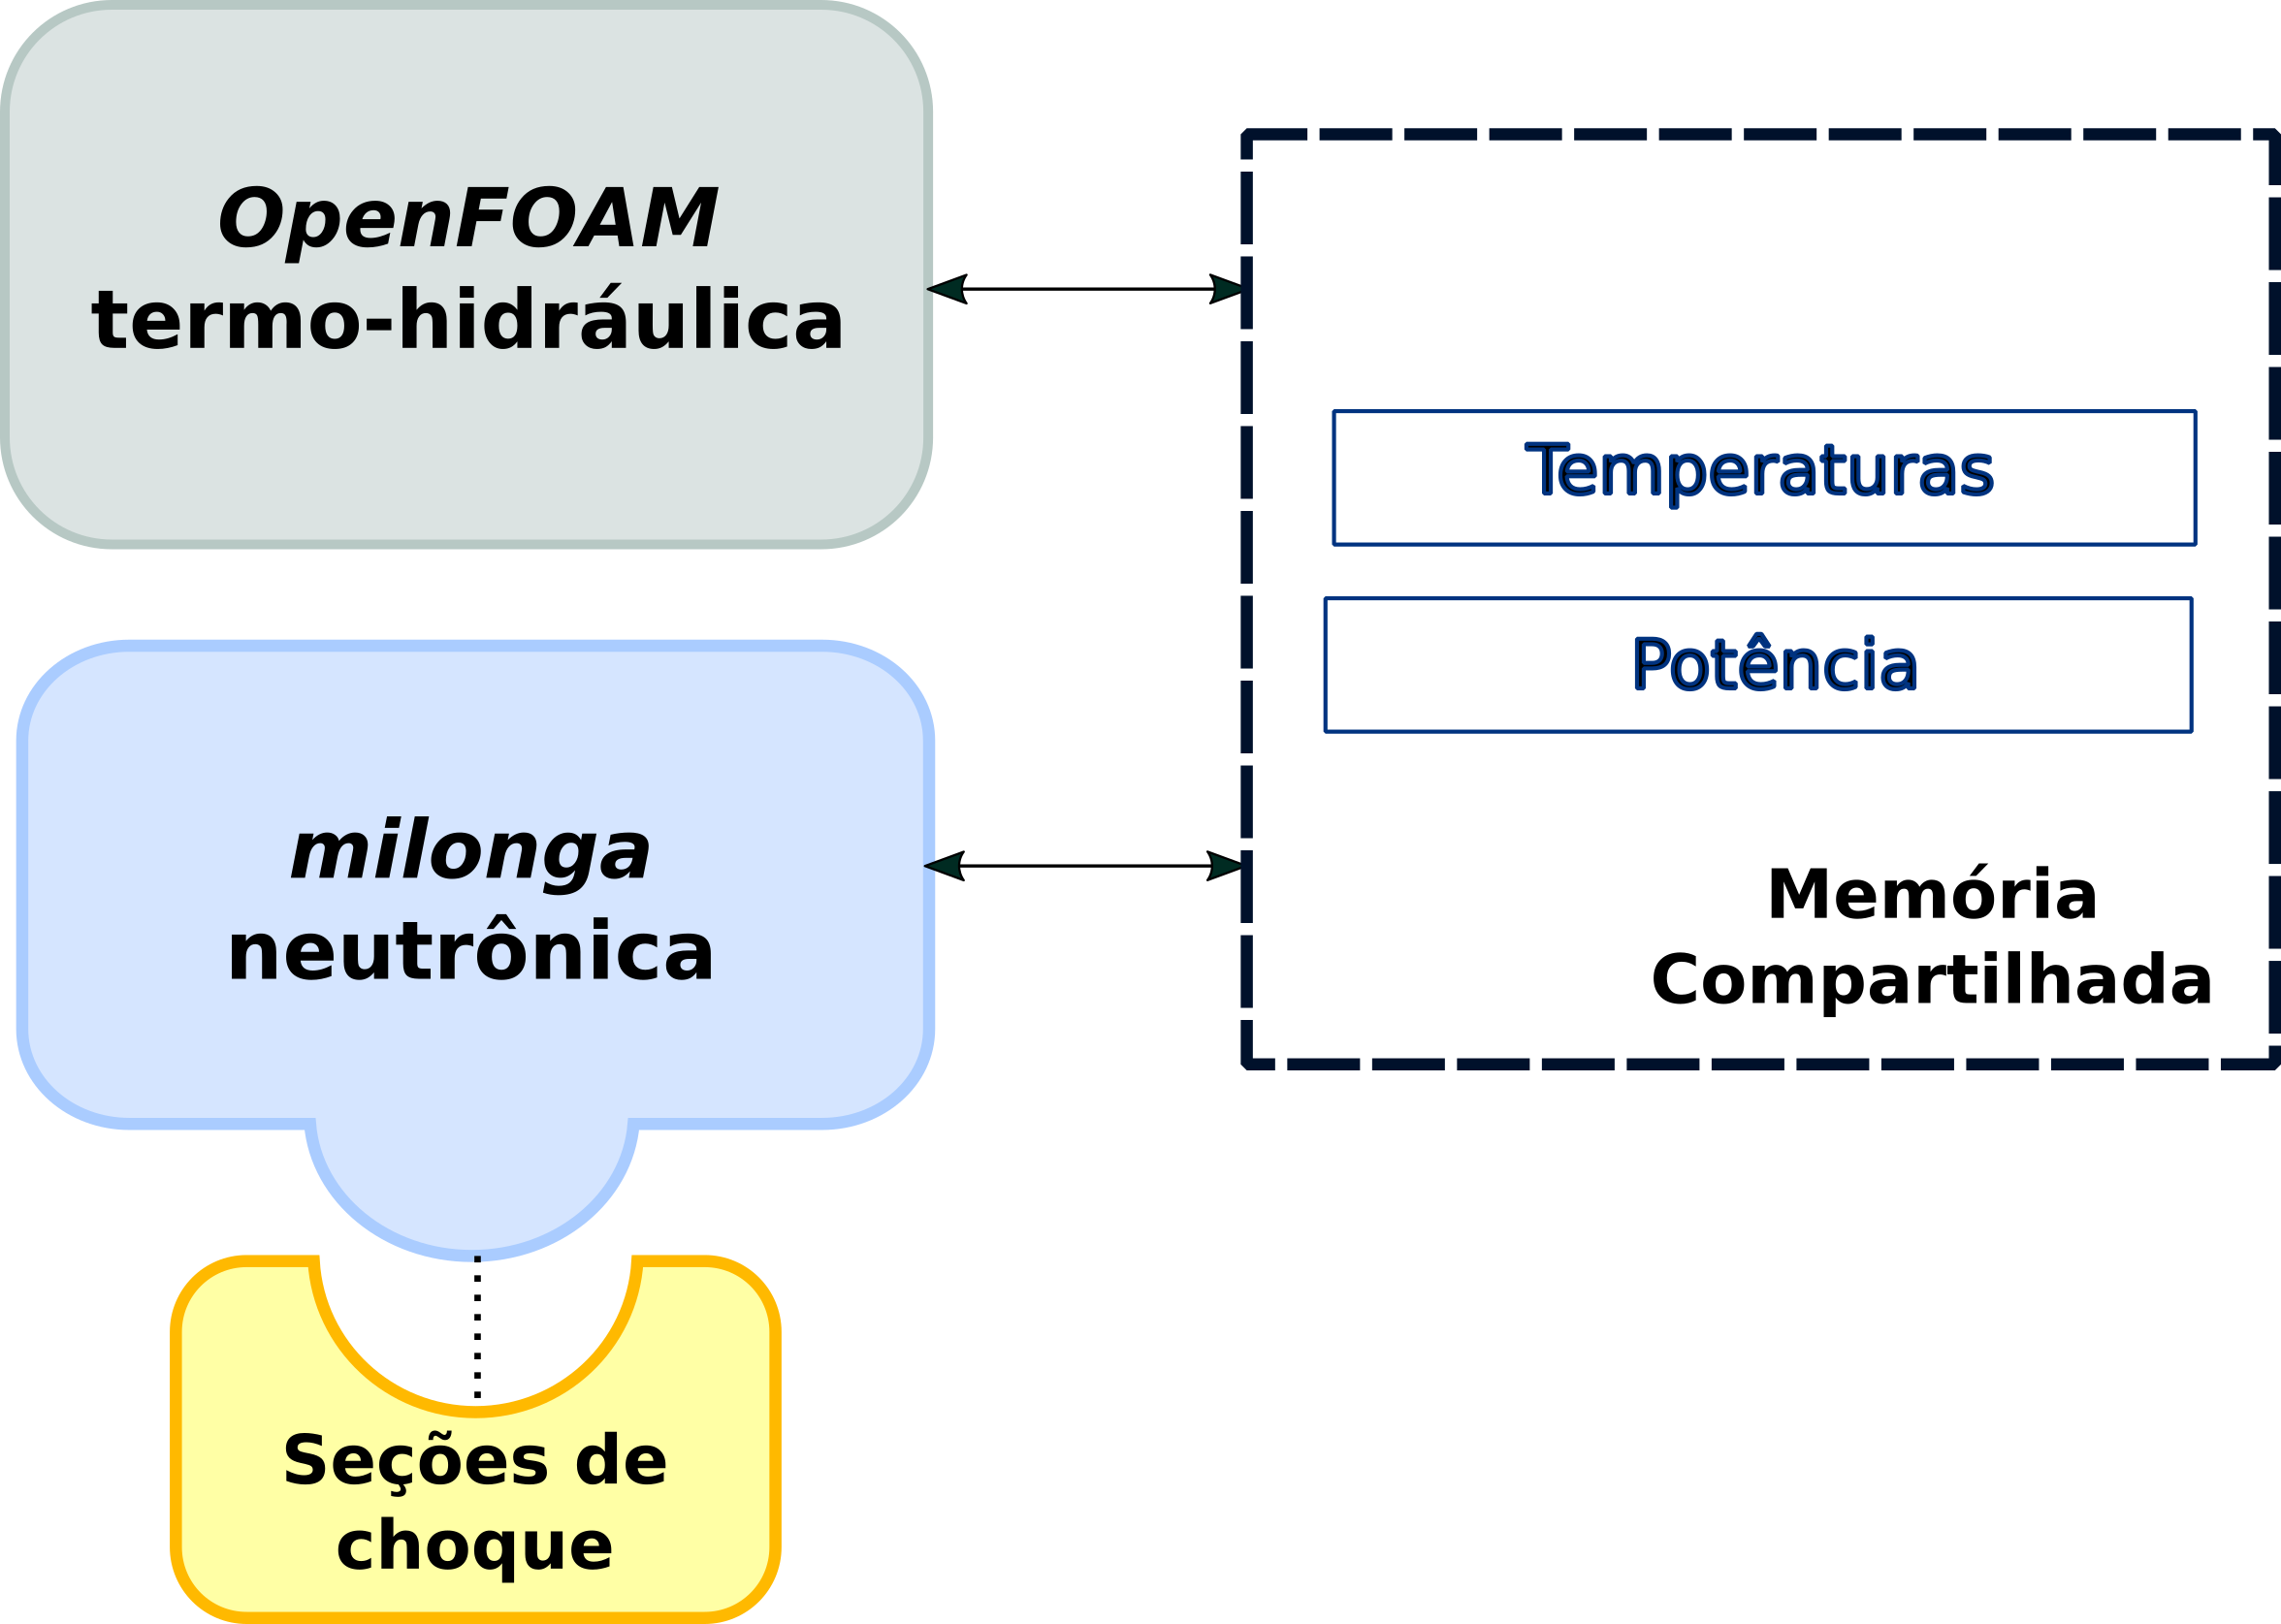
\includegraphics[scale=0.6]{figuras/metodologia2.png}
  \label{metodoetapas}
%  \legend{Fonte: autor}
\end{figure}

Como apresentado no capítulo \ref{chap:rev}, o acoplamento, no contexto desta dessa tese, é a execução
de cálculos termo-hidráulicos utilizando a potência obtida pelo código de neutrônica que, por sua vez,
utiliza as temperaturas dos materiais calculadas pela termo-hidráulica para re-calcular seções de choque
e outros parâmetros neutrônicos de modo a calcular o fluxo de nêutrons e potência no combustível.

As características não-usuais desse sistema são listadas abaixo:

\begin{itemize}
\item Dois \textit{softwares} independentes interligados;
\item Uso de memória compartilhada para comunicação entre dois diferentes códigos;
\item Natureza aberta das licenças de utilização de ambos os programas (item fundamental para
  o acesso, modificação e utilização do código-fonte de ambos);
\end{itemize}

Nas próximas seções serão apresentadas em seus detalhes cada uma destas características que
permitiram o desenvolvimento de um sistema multi-física.

\section{Conceitos}
\label{sec:conc}

Como discutido anteriormente, nesta seção serão apresentados brevemente os conceitos sobre os quais
foi construído o sistema acoplado.

\subsection{Multi-tarefa}
\label{subsec:mt}

Multi-tarefa é a capacidade dos sistemas operacionais de executar distintas tarefas ao mesmo tempo.
Talvez possa parecer corriqueira tal observação nos dias de hoje. Entretanto, há pouco mais de vinte
anos, a maioria dos sistemas operacionais usados em computadores pessoais não ofereciam esta
possibilidade. Em alguns casos, o que se chamou de multi-tarefa preemptiva, o usuário era capaz de
carregas distintas tarefas em memória. Contudo, apenas uma era executada por vez.

Nos sistemas computacionais atuais, em especial no sistema Linux, utilizado para o desenvolvimento
do sistema multi-física desta tese, é possível executar diversas tarefas ao mesmo tempo. Não só isso,
como há um sistema padrão de execução que permite a comunicação entre programas distintos. Diferente
de um sistema de \textit{threads} \cite{Posix}, em que todos os programas lançados enxergam a mesma
porção de memória, no sistema Linux cada programa tem acesso exclusivo à memória alocada para si.
Tudo isso acontece sob gerenciamento do sistema operacional.

A metodologia utilizada neste acoplamento, prevê a execução separada dos programas de termo-hidráulica
e neutrônica. Os detalhes e os algoritmos desta comunicação serão apresentados em detalhes oportunamente.
Por agora, é suficiente saber que os programas são lançados separadamente, cada qual utilizando a memória
alocada para si separadamente, sem que outros programas possam acessá-la. Dessa forma, era necessário
desenvolvier um sistema de comunicação entre os códigos de neutrônica e termo-hidráulica.

\subsection{Memória compartilhada}
\label{subsec:mc}

Memória compartilhada (ou \textit{Shared-memory}) é uma região de memória que pode ser simultaneamente
acessada por programas executando em diferentes espaços de usuário. O sistema operacional Linux
oferece por padrão ferramentas para acesso, leitura, alocação, liberação e vários outras operações
para utilização de memória compartilhada. Além disso, oferece também ferramentas para sincronização
deste acesso, uma vez que como há mais de um programa acessando os mesmos dados, podem ocorrer
condições de corrida \footnote{\textit{Race condition} é o nome dado aos problemas e erros introduzidos
  nos cálculos quando \textit{threads} ou programas acessam uma porção de memória sem saber que os dados
foram modificados, afetando o estado atual destes.}.

Há diferentes técnicas para evitar condições do corrida. Dentre elas, uma das mais simples e
largamente empregada, é o uso de semáforos, inclusive usada nesta tese.
Um programa ou \textit{thread}, antes de acessar a memória
verifica se esta está livre para ser acessada. Se sim, altera o valor do semáforo enquanto opera na
memória, voltando a alterá-lo para ``livre'' ao terminar. Caso outro programa ou \textit{thread}
necessite acessar a mesma porção de memória, encontrará o semáforo em condição negativa e aguardará
um determinado tempo (definido pelo sistema operacional ou pelo próprio usuário) até tentar novamente.
Com isso, fica garantida a não-corrupção dos dados.

Deve-se dizer que há implicações negativas no uso de semáforos para controle de acesso à memória,
como por exemplo, queda de desempenho dos sistemas, em especial quando há um número grande
de programas acessando a memória compartilhada. Entretanto, a análise da possível degradação
de desempenho causada por controle de concorrência entre programas não é escopo desta tese.

\subsection{\textit{Software} livre}
\label{subsec:sl}

Muito já se disse sobre \textit{software} livre, suas características e suas licenças, como na
seção \ref{sec:intsl}. Nesta sub-seção, o objetivo se restringe às vantagens do acesso ao
código-fonte.

Ambos os códigos usados no sistema acoplado, possuem a capacidade de serem acoplados sem alterações
em seus códigos-fonte. O \textit{milonga}, em especial, já foi desenvolvido com a possibilidade
de acoplamento em mente. Portanto, oferece mais de uma forma de comunicação de dados, como por exemplo:
arquivos texto, arquivos binários e, inclusive, de forma nativa, uso de memória compartilhada.

O \textit{OpenFOAM}, entretanto, em um cenário de código fechado, só ofereceria uma forma de
acoplamento. De acordo com sua implementação, um termo-fonte só pode ser lido a cada início de
simulação. Seria, portanto necessário fazer com que o \textit{mionga} lesse os dados de temperatura
da saída do \textit{OpenFOAM}, escrevesse uma distribuição de potências em formato de entrada
para o \textit{OpenFOAM} e que este fosse novamente executado do zero. Todo esse processo, deveria
ser controlado por um \textit{script} de execução.

Apesar de soar rudimentar, está é a forma de acoplamento mais comumente empregada.
Mesmo com severo comprometimento de desempenho se comparada a compartilhamento de
memória, muitas vezes esta é a única forma de acoplamento quando o código-fonte não
está disponível \cite{Hummel2016}.

\section{Ferramentas}
\label{sec:ferr}

Na seção anterior, foram brevemente descritos os conceitos sobre os quais foi construído
o sistema acoplado desenvolvido nesta tese. Este
sistema utiliza dois diferentes programas de computador. Cada um deles
realiza um conjunto de cálculos separadamente e compartilham os dados necessários aos cálculos do outro.

Apesar de desenvolvidos separadamente e com objetivos diferentes, algumas características comuns - além
do fato de serem ambos \textit{software} livre - permitiram seu uso acoplado. Ambos utilizam métodos de
discretização de domínio compatíveis e possuem a capacidade de lidar com um formato aberto de arquivos de descrição de malhas. Essas características tornam possível o desenvolvimento de um acoplamento sem mapeamento, ou seja, ambos os códigos trabalham no mesmo domínio, resolvendo suas respectivas equações no mesmo nível de detalhes espaciais que seu oposto.

%São dedicadas subseções a cada característica deste acoplamento definida anteriormente como não-usual.

As próximas sub-seções exploram as características destes programas que permitiram desenvolver
a metodologia neste acoplamento. São também apresentados os principais desenvolvimentos técnicos
relacionados a metodologia desenvolvida.

\subsection{Termo-hidráulica: \textit{OpenFOAM}}
\label{subsection:openfoam}

O \textit{OpenFOAM} é um pacote para simulação numérica de Mecânica
do contínuo desenvolvido com base em orientação a objetos em linguagem $C++$ .
Do ponto de vista de Engenharia de Software, sua modularidade e flexibilidade são vantagens
em relação a outros códigos monolíticos  \cite{Jasak2007}. Sua implementação em componentes para manipulação de malhas, suporte
à solução de sistemas lineares, operadores de discretização e modelos físicos em forma de bibliotecas o tornam
um sistema CFD completo, aberto e gratuito. É utilizado em uma grande variedade
de aplicações, desde a solução de escoamentos complexos envolvendo reações químicas, turbulência e
transferência de calor até acústica, mecânica dos sólidos e eletromagnetismo. 

\textit{OpenFOAM} implementa um manipulador de malhas poliédrico, no qual células são descritas a partir
de um conjunto de faces fechando um volume. As faces, por sua vez, são formadas por uma lista de pontos
em suas coordenadas cartesianas e armazenados como vetores. Esta implementação é independente da discretização
usada \cite{Jasak2009}. Entretanto, as principais classes que herdam as funcionalidades das malhas implementam o método de
volumes finitos. Sendo assim, pode-se dizer que o \textit{OpenFOAM} é um sistema de CFD baseado em volumes
finitos.

Além dos componentes dedicados a operações sobre o domínio, o \textit{OpenFOAM} oferece um conjunto variado
de programas independentes chamados \textit{solvers}. Estes \textit{solvers} são dedicados à solução de
problemas físicos específicos. Para isto, utilizam outros elementos disponíveis no conjunto do
\textit{OpenFOAM}. O problema físico a ser resolvido nesta tese, especificamente do ponto de vista
termo-hidráulico, é o da solução de troca de calor conjugada entre sólidos e
fluidos distintos. Um dos \textit{solvers} que o \textit{OpenFOAM} possui com esse propósito é o
\texttt{chtMultiRegionSimpleFoam} \cite{OpenFOAM2015}.

Este \textit{solver} funciona para problemas em estado estacionário e para
fluidos compressíveis. A modularidade do \textit{OpenFOAM}
fica clara na forma como o \textit{solver} interage com os outros módulos: para regiões sólidas,
são utilizados modulos de propriedades termo-físicas específicos para sólidos. Por sua vez, para
fluidos são oferecidos outros módulos com implementações relativas a propriedades de fluidos.
Outro exemplo é a utilização de turbulência: caso o usuário estabeleça que seu escoamento é laminar,
o módulo para escoamentos laminares é utilizado. Caso o escoamento seja turbulento, o usuário pode
escolher entre implementações de diferentes modelos de turbulência.

O \textit{solver} utilizado permite escolher entre energia interna e entalpia para a solução
da equação da energia, de acordo com o módulo termodinâmico escolhido. Na implementação do
problema acoplado, foi usada entalpia. O modelo de turbulência utilizado foi o $\kappa-\epsilon$
\cite{Launder1974}.
%Mais detalhes as características do escoamento simulado e do modelo de turbulência serão
%discutidos no capítulo \ref{chap:aplicacao} e sub-seção \ref{subsec:turb}, respectivamente.

\subsubsection{Implementação: \texttt{thesisCoupledFoam}}
\label{subsec:detth}
Na seção \ref{sec:th} foram apresentadas as bases teóricas do problema termo-hidráulico.
Nesta sub-seção, são
descritas as alterações diversas promovidas no \textit{solver} original do \textit{OpenFOAM}
que foi chamado \texttt{thesisCoupledFoam}.

A principal alteração feita no \textit{solver} originalmente implementado foi a adição de um termo-fonte.
Esta alteração permite a geração de calor no sólido, útil tanto no problema acoplado
quanto numa eventual simulação isolada em que se deseje geração de
calor\footnote{A partir da versão 2.2, o \textit{OpenFOAM} introduziu em alguns dos seus
\textit{solvers}, incluindo o \texttt{chtMultiRegionSimpleFoam} a possibilidade de definição
de termo-fonte via \texttt{fvOptions}. Isso permite alteração da física do problema em
tempo de execução. Infelizmente, a forma de implementação desta funcionalidade não atendia uma
utilização do \textit{solver} de forma acoplada.}. Isso foi feito acrescentando-se uma estrutura
do tipo campo escalar volumétrico, estrutura de dados utilizada pelo \textit{OpenFOAM},
para armazenar os valores de potência a serem usados. Sendo assim, na sua inicialização,
o \textit{solver} modificado busca, além dos arquivos padrão para as grandezas calculadas, um
arquivo chamado \texttt{Q} que deve conter o campo volumétrico de potências em $W/m^3$. Caso
este arquivo não seja encontrado, é inicializado com valores nulos para o termo-fonte.

O trecho de código em que a leitura do campo volumétrico para a potência é feita
é apresentado na listagem \ref{lst:Q}.

\begin{lstlisting}[caption={Leitura/criação do campo volumétrico de potências.}\label{lst:Q}]
  PtrList<volScalarField> qVol(solidRegions.size());

  // Read Q if it exists. If not, create a null (zero) volScalarField
  IOobject Qfile("Q", runTime.timeName(), solidRegions[i],
                 IOobject::READ_IF_PRESENT, IOobject::AUTO_WRITE);

  // Must check it before creating the field
  if(Qfile.headerOk())
  {
    // Create a qvol field from dictionary
    qVol.set(i, new volScalarField (Qfile, solidRegions[i]));
  }
  else
  {
    // If file is not there, create a new IOobject
    // setting the dimensions of the field
    qVol.set(i,
    new volScalarField(IOobject
                          ("Q", runTime.path(), solidRegions[i], IOobject::NO_READ,
                              IOobject::AUTO_WRITE), solidRegions[i], dimensionedScalar
                          ("2", dimensionSet(1, -1, -3, 0, 0), scalar(0.0))
                          )
                      );
  }
\end{lstlisting}

Na linha $1$, é criada uma lista de ponteiros para campos escalares volumétricos. Essa estrutura
retém as referências para os campos volumétricos de potencias de todas as regiões sólidas. Na
presente implementação, apenas a região com nome \textbf{``fuel''} pode ter um valor não nulo
para o campo de potências. Na linha $4$ cria-se um objeto de entrada e saída de acordo com o
arquivo \textbf{``Q''}. Se o
objeto criado tiver o cabeçalho correto (linha $8$) é criada uma entrada na lista de referências com os
dados do arquivo (linha $11$). Caso contrário, se um arquivo mal-formado for encontrado ou
não for encontrado o arquivo, é criado um campo volumétrico escalar com valores nulos nas dimensões
esperadas (linhas $17$ a $23$). A partir deste ponto, o campo escalar volumétrico \textbf{``Q''}
está disponível para ser usado.

A criação do campo escalar volumétrico de potências é feito na inicialização dos campos dos materiais
sólidos, anterior ao algoritmo de solução. O algoritmo de solução usado é o SIMPLE
\textit{(Semi-Implicit Method for Pressur-Linked Equations}). Este algoritmo funciona
estimando um valor inicial para o cálculo da pressão e então fazendo correções no valor
estimado \cite{Versteeg2007}. Esse procedimento é repetido até que se chegue a um valor
aceitável dentro das condições de parada. Lembrando que este procedimento é feito para
a solução do escoamento. O \textit{solver} resolve separadamente cada região de acordo com seu
tipo, fluida ou sólida, tudo isso dentro da iteração do algoritmo SIMPLE.

Um fragmento do laço de iterações do algortimo SIMPLE é apresentado na listagem \ref{lst:simple}.

\begin{lstlisting}[caption={Fragmento do laço do algoritmo SIMPLE.}\label{lst:simple}]
  while (runTime.loop())
  {
    nIterations++;

    forAll(fluidRegions, i)
    {
      // Fluid regions loop: removed for the sake of clarity
    }
    
    forAll(solidRegions, i)
    {
      #include "setRegionSolidFields.H"
      #include "readSolidMultiRegionSIMPLEControls.H"
      #include "solveSolid.H"
      
      runTime.write();
    }
\end{lstlisting}

O controle da simulação é feito pelo objeto \texttt{runTime}, responsável por avaliar resíduos
e outras condições de parada. As regiões definidas como fluidas são resolvidas num laço (linha $5$)
e então são resolvidas as equações para as regiões sólidas (linha $10$). O \textit{OpenFOAM} utiliza-se
de uma diretiva de inclusão (linhas $12$ a $14$) para adicionar ao código-fonte o conteúdo de outros
arquivos definidos pelos nomes. Isso é feito com o objetivo de deixar o código-fonte mais legível como
também de evitar re-escrita de código, já que muitos dos arquivos incluídos são comuns a outros
\textit{solvers}. Um desses arquivos (linha $14$) é o que contém as equações a serem resolvidas para
a região sólida. É nele que o campos escalar volumétrico \textbf{``Q''} é utilizado. Um fragmento
do arquivo de solução de sólidos é apresentado na listagem \ref{lst:solvesolid}.

\begin{lstlisting}[caption={Fragmento do laço do algoritmo SIMPLE.}\label{lst:solvesolid}]
  {
    for (int nonOrth=0; nonOrth<=nNonOrthCorr; nonOrth++)
    {
      fvScalarMatrix hEqn
      (
      - fvm::laplacian(betav*alpha, h, "laplacian(alpha,h)")

      // Source-term added to que equation
      - Q
      );

      hEqn.relax();
      hEqn.solve();
    }
  }
\end{lstlisting}

Dentro de um laço interno para correção de não-ortogonalidade, é definida a matriz de solução
referente a entalpia (linha $4$). Como argumentos do objeto matriz sendo criado, é adicionado
o termo-fonte \textbf{``Q''} (linha $9$). Estas são as principais
modificações no código-fonte do \textit{solver} para
acrescentar o termo-fonte à equação do calor no sólido.

Outra modificação importante é a adição de estruturas de dados capazes de fazer a comunicação
por memória compartilhada.

% ------------------------------------------------------------------------------------------------

% codigo e explicação de shared memory.

% -------------------------------------------------------------------------------------------------
Espera-se, ao apresentar algumas das implementações feitas em fragmentos do código-fonte
do \textit{OpenFOAM}, familiarizar o leitor com o formato interno do \textit{OpenFOAM}
e alguns detalhes de como se deu, na prática, o proposto na metodologia de acoplamento
desenvolvida nesta tese. Entretanto, o objetivo deste capítulo é na
explicação da metodologia de acoplamento. Portanto, a implementação da comunicação
entre \textit{OpenFOAM} e \textit{milonga}
dentro do \textit{solver} \texttt{thesisCoupledFoam} e todos os detalhes menores da implementação
estão disponíveis no anexo \ref{anx:codigo} onde está listado o código-fonte completo
da implementação desta tese. Fica o leitor convidado a ler o código-fonte para obter todos
os detalhes técnicos.

Uma característica particular do acoplamento proposto, é o uso de malhas iguais para neutrônica
e termo-hidráulica. São raros os acoplamentos com essa característica na literatura \cite{Jareteg2014}
e suas vantagens são, principalmente:

\begin{itemize}
\item Solução multi-física no mesmo nível de detalhes\footnote{Neste trabalho, se considera ``nível de detalhes'' o  mesmo grau de discretização para ambos os problemas. O conceito pode ser estendido se for
  considerado o erro relativo dos cálculos em cada problema. Não é este o caso.};
\item Evita-se o mapeamento entre malhas que, no caso de malhas não-estruturadas, além de ser um problema de
  geometria computacional não-trivial , eventuais soluções podem acrescentar
  erros entre células \cite{Kraevoy2004}.
\item Criação de vetores shared-memory e semáforos
\end{itemize}





% -----------------------------------------------------------------------------------------------------

\subsection{Neutrônica: \textit{milonga}}
\label{subs:milonga}

\subsubsection{Equações}

\begin{itemize}
\item Adição do termo-fonte (1 alteração na equação do sólido: colocar equação já no formato OpenFOAM)
\end{itemize}

\section{\textit{Shared-memory}}

\textit{Shared-memory} (ou memória compartilhada) é a memória de computadores que pode ser
acessada simultaneamente por múltiplos programas com o objetivo de oferecer comunicação entre
eles evitando cópias redundantes \cite{Robbins2003}. É, ainda, uma forma eficiente de passagem de dados entre programas
ou processos. A interface POSIX (\textit{Portable Operating System Interface}) é padrão especificado pela
\textit{IEEE Computer Society} para garantir a compatibilidade entre diferentes sistemas operacionais. Neste padrão
está definida uma API (\textit{Application programming interface}), ambientes de comando e cojuntos de utilitários
para compatibilidade de \textit{software} entre sistemas operacionais \cite{Atlidakis2016}.

Essa padronização permite os dois diferentes códigos usados no acoplamento utilizem-se das extensões POSIX nas
suas linguagens de programação para ler, escrever e se comunicar através do uso de memória-compartilhada.

%É desconhecido na literatura o uso de memória compartilhada (\textit{shared-memory} para
%acoplamento neutrônico e termo-hidráulico.





%\section{Malha}

%\begin{figure}[htb]
%  \caption{Malha e regiões, vista superior.}
%  \centering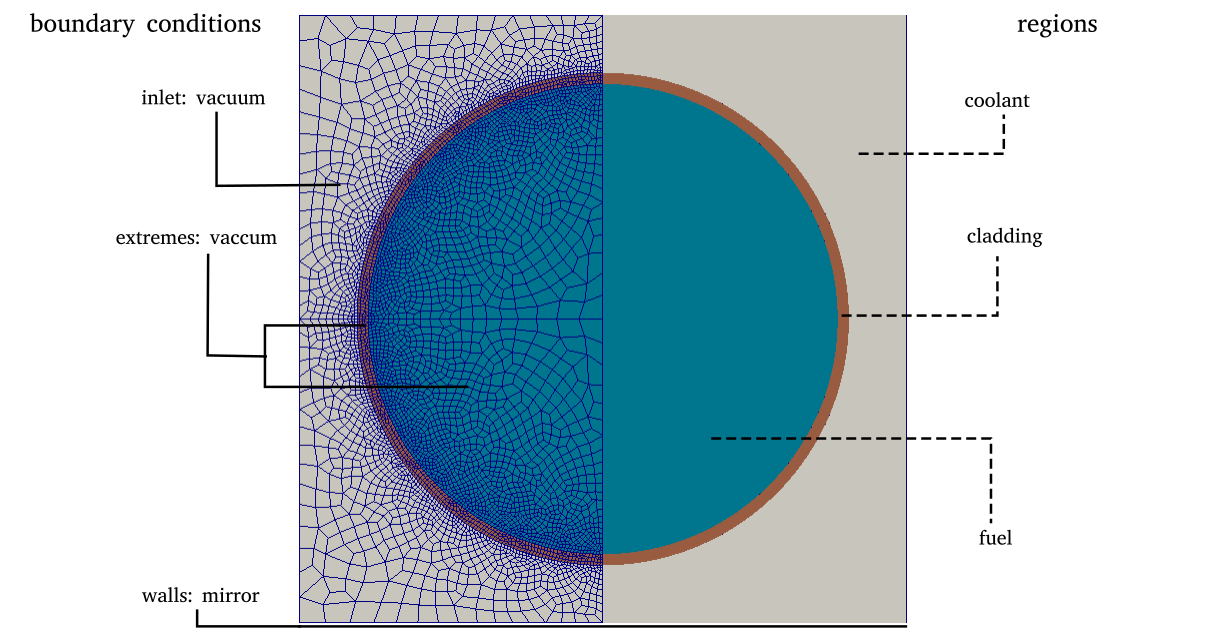
\includegraphics[scale=0.5]{figuras/regions_neutronica_malha_e_sem.png}
%  \label{regions_malha}
%  \legend{Fonte: autor}
%\end{figure}

%\section{Condições de contorno}


\section{Acoplamento} % Algoritmos


\subsection{Algoritmo neutrônica}

\begin{figure}[htb]
  \caption{Algoritmo neutrônica.}
  \centering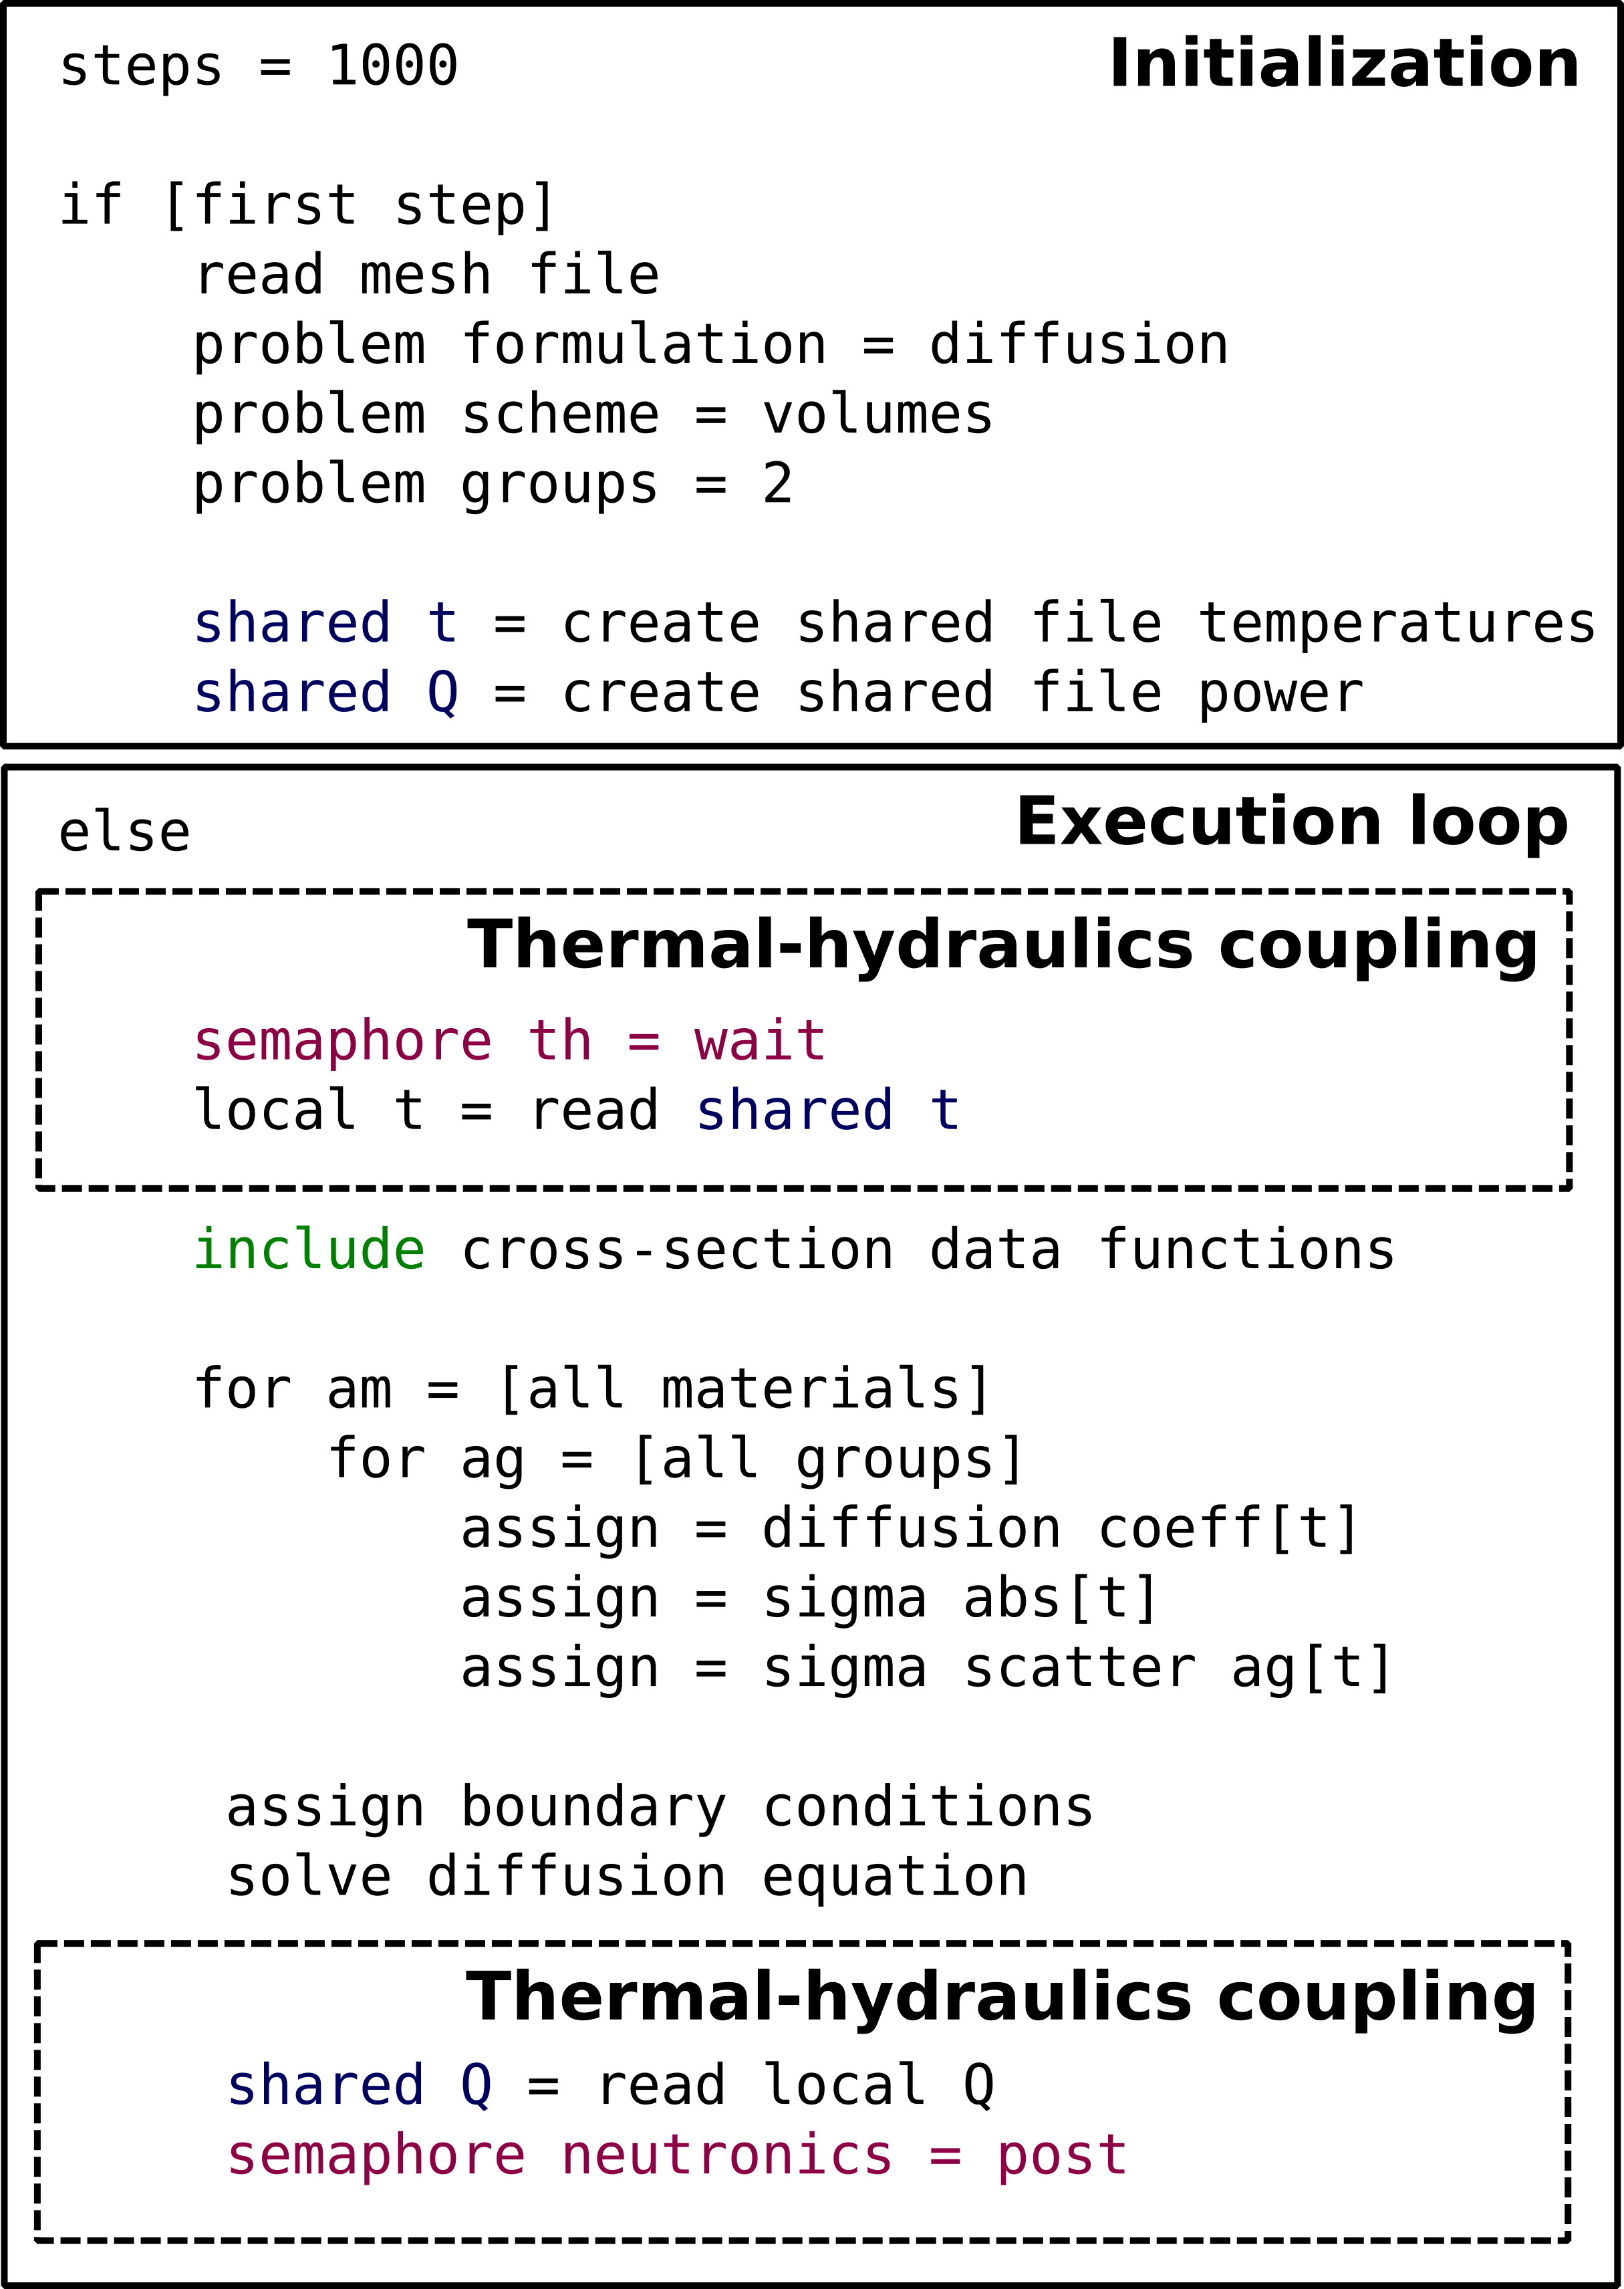
\includegraphics[scale=0.5]{figuras/algoritmos_milonga.png}
  \label{algo_neutronica}
  \legend{Fonte: autor}
\end{figure}

\subsection{Algoritmo termo-hidráulica}
\label{subsec:th}

\begin{figure}[htb]
  \caption{Algoritmo termo-hidráulica.}
  \centering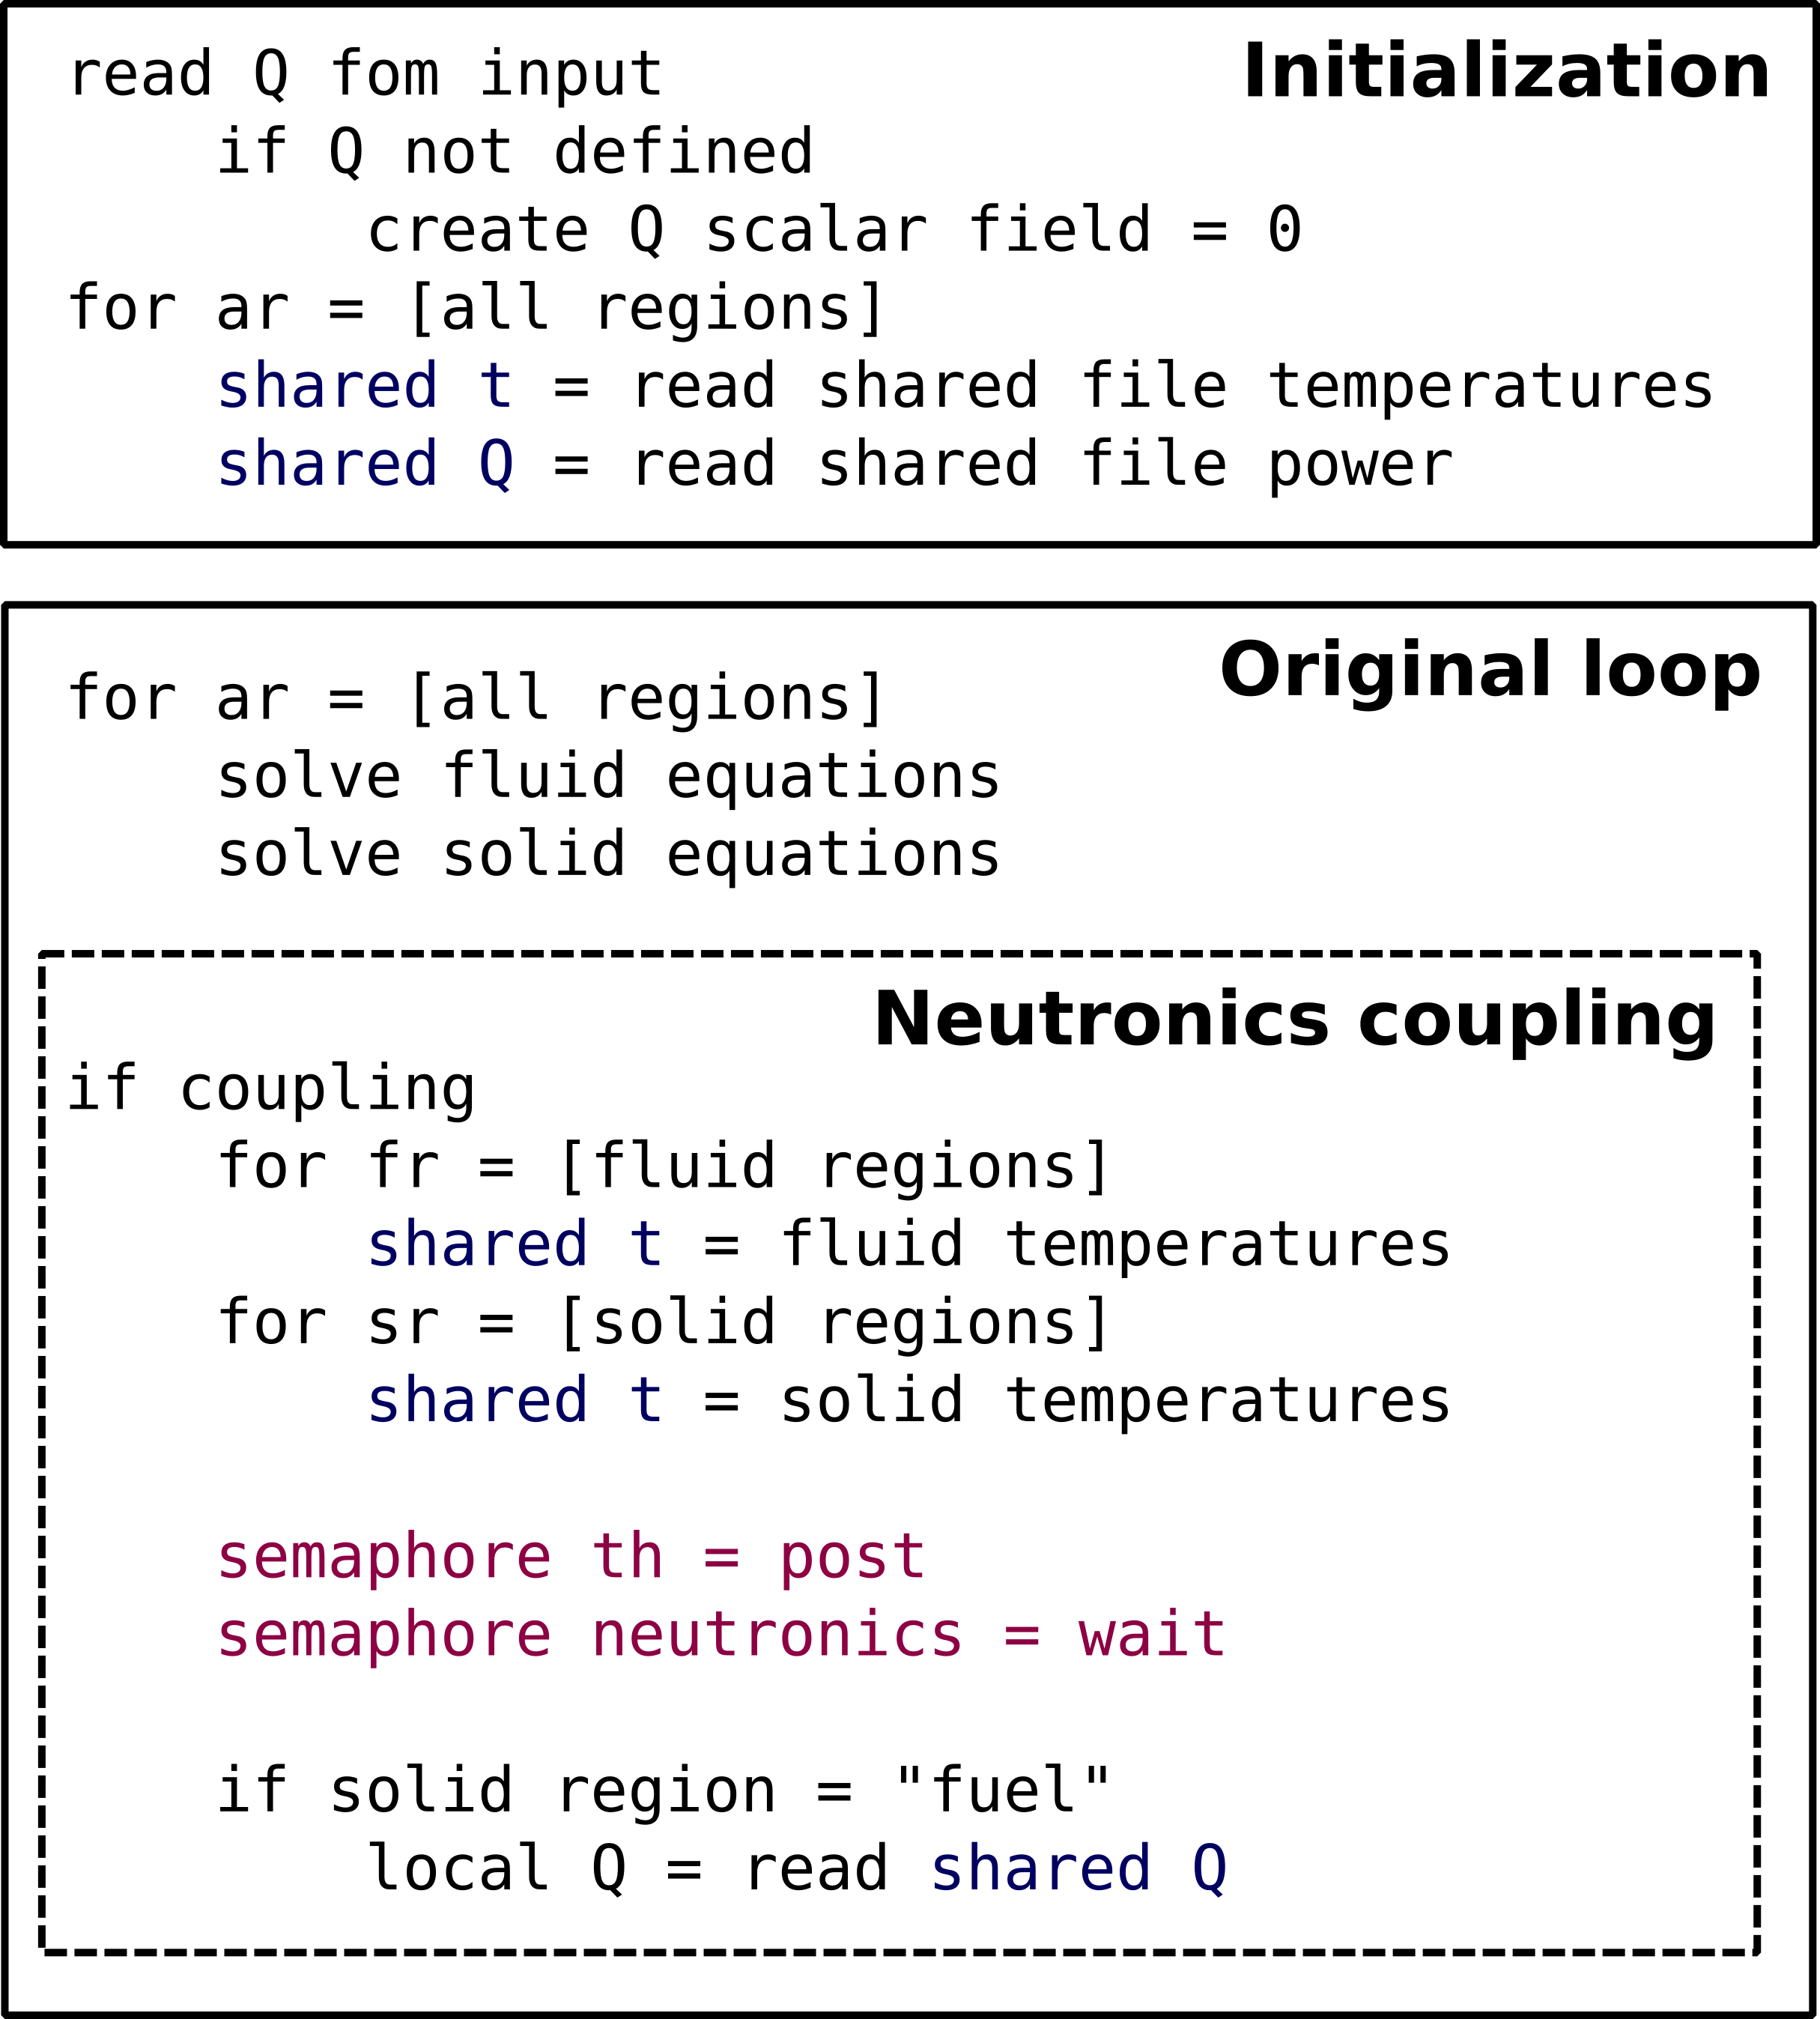
\includegraphics[scale=0.5]{figuras/algoritmo_openfoam.png}
  \label{algo_th}
  \legend{Fonte: autor}
\end{figure}



%Modelada uma geometria idêntica à representada na malha utilizada pelo \textit{OpenFOAM},
%foram feitas simulações da neutrônica pelo Serpent com objetivo de obter as seções
%de choque em dois grupos a serem usadas na solução da aproximação por difusão dos nêutrons
%pelo \textit{milonga}.

%Na saída do Serpent são dados constantes de groups homogeneizadas (neste caso, com espectro
%corrigido para fugas pelo método B1 \textbf{CITAR}) e outros parâmetros de interesse para
%a modelagem por difusão como, por exemplo, os coeficientes de difusão para cada grupo já
%calculados.

%Como todos os elementos do desenvolvimento estão relacionados entre si, sempre que
%julgado oportuno para a clareza do entendimento, os conceitos desenvolvidos em cada
%seção poderão ser apresentados conjuntamente. De fato, uma vez que o problema multifísica
%(ou acoplamento) nada mais é do que a solução conjunta de dois problemas que são,
%usualmente, resolvidos separadamente, é natural como definir, modelar e resolver os
%dois problemas separadamente.

%De acordo com as definições de problemas acoplados apresentadas
%no capítulo \ref{chap:rev}, ao resolver os problemas neutrônico e termo-hidráulico
%separadamente, o acoplamento ainda pode ser considerado implícito de acordo com, já que a troca de informações entre os problemas ocorre ao nível de termos completos,
%e não em condições de contorno. É importante dizer que essa nomeclatura para as formas
%de acoplamento não é unânime na literatura \cite{Ivanov2007}.

%Deve estar claro que a metodologia a ser descrita trata do ciclo de desenvolvimento
%do \textit{software} acoplado. Apesar de ser possível considerar as simulações e
%os processos de pré-processamento e pós-processamento, tanto termo-hidráulicos quanto
%neutrônicos, optou-se por tratar destas etapas exclusivamente na seção de validação e,
%quando pertinente, nos resultados obtidos.


%Na figura \ref{metodoetapas} são apresentadas as relações entre os diferentes elementos
%do sistema acoplado.





